\documentclass{article}

\usepackage[utf8]{inputenc}
\usepackage[brazilian]{babel}
\usepackage{graphicx}
\usepackage{float}
\usepackage[pdftex]{hyperref}
\usepackage{epstopdf}
\usepackage{etoolbox}
\usepackage{amsmath}
\usepackage{amsfonts}
\usepackage{amssymb}
\usepackage{caption}
\usepackage{subcaption}
\usepackage{setspace}
\usepackage{tikz}

\patchcmd{\thebibliography}{\section*}{\section}{}{}
\newcommand{\R}{\ensuremath{\mathbb{R}}}
\newcommand{\Prob}{\ensuremath{\mathbb{P}}}
\newcommand{\K}{\ensuremath{\mathbb{K}}}
\newcommand{\U}{\ensuremath{\mathbb{U}}}
\newcommand{\N}{\ensuremath{\mathbb{N}}}
\newcommand{\Lg}{\ensuremath{\mathbb{L}}}
\newcommand{\T}{\ensuremath{\rm Tr}}
\newcommand{\sg}{{\sigma(x_k)}}

\newcommand{\G}{\ensuremath{\mathcal{G}}}
\newcommand{\F}{\ensuremath{\mathcal{F}}}
\newcommand{\C}{\ensuremath{\mathcal{C}}}
\newcommand{\E}{\ensuremath{\mathcal{E}}}
\newcommand{\Hn}{\ensuremath{\mathcal{H}}}
%\newcommand{\Hoo}{\ensuremath{\mathcal{H}_\infty}}
\newcommand{\Hop}{\ensuremath{\mathcal{H}_{op}}}
% --------------------------------------------------
\newtheorem{theo}{Teorema}
\newtheorem{exa}{Exemplo}
\newtheorem{lemm}{Lema}
\newtheorem{coro}{Corolário}
\newtheorem{defn}{Definição}[section]

%opening


\begin{document}
\input{capa.tex}

\onehalfspacing
\section{Objetivos} 
O objetivo desse experimento é a identificação da função de transferência de sistemas eletrônicos de terceira ordem. Nesse experimento nós medimos a resposta à uma onda quadrada de uma planta semi-desconhecida e através da saída de cada estágio conseguimos estimar os parâmetros de sua função de transferência. 
	
\section{Determinação dos parâmetros da função de transferência}
Utilizando a plataforma Elvis e o lab view aplicamos uma onda quadrada na entrada do circuito $PLT06$ que nos foi disponibilizado durante o experimento, de maneira a reproduzir o sinal de entrada do pré-roteiro. Obtivemos medições da saída da planta em cada estágio que serão analisados nas seções subsequentes.

\subsection{1$^o$ Estágio}
A resposta do $1^o$ estágio da planta pode ser vista na figura \ref{fig:saida1}.
\begin{figure}[H]
	\centering
	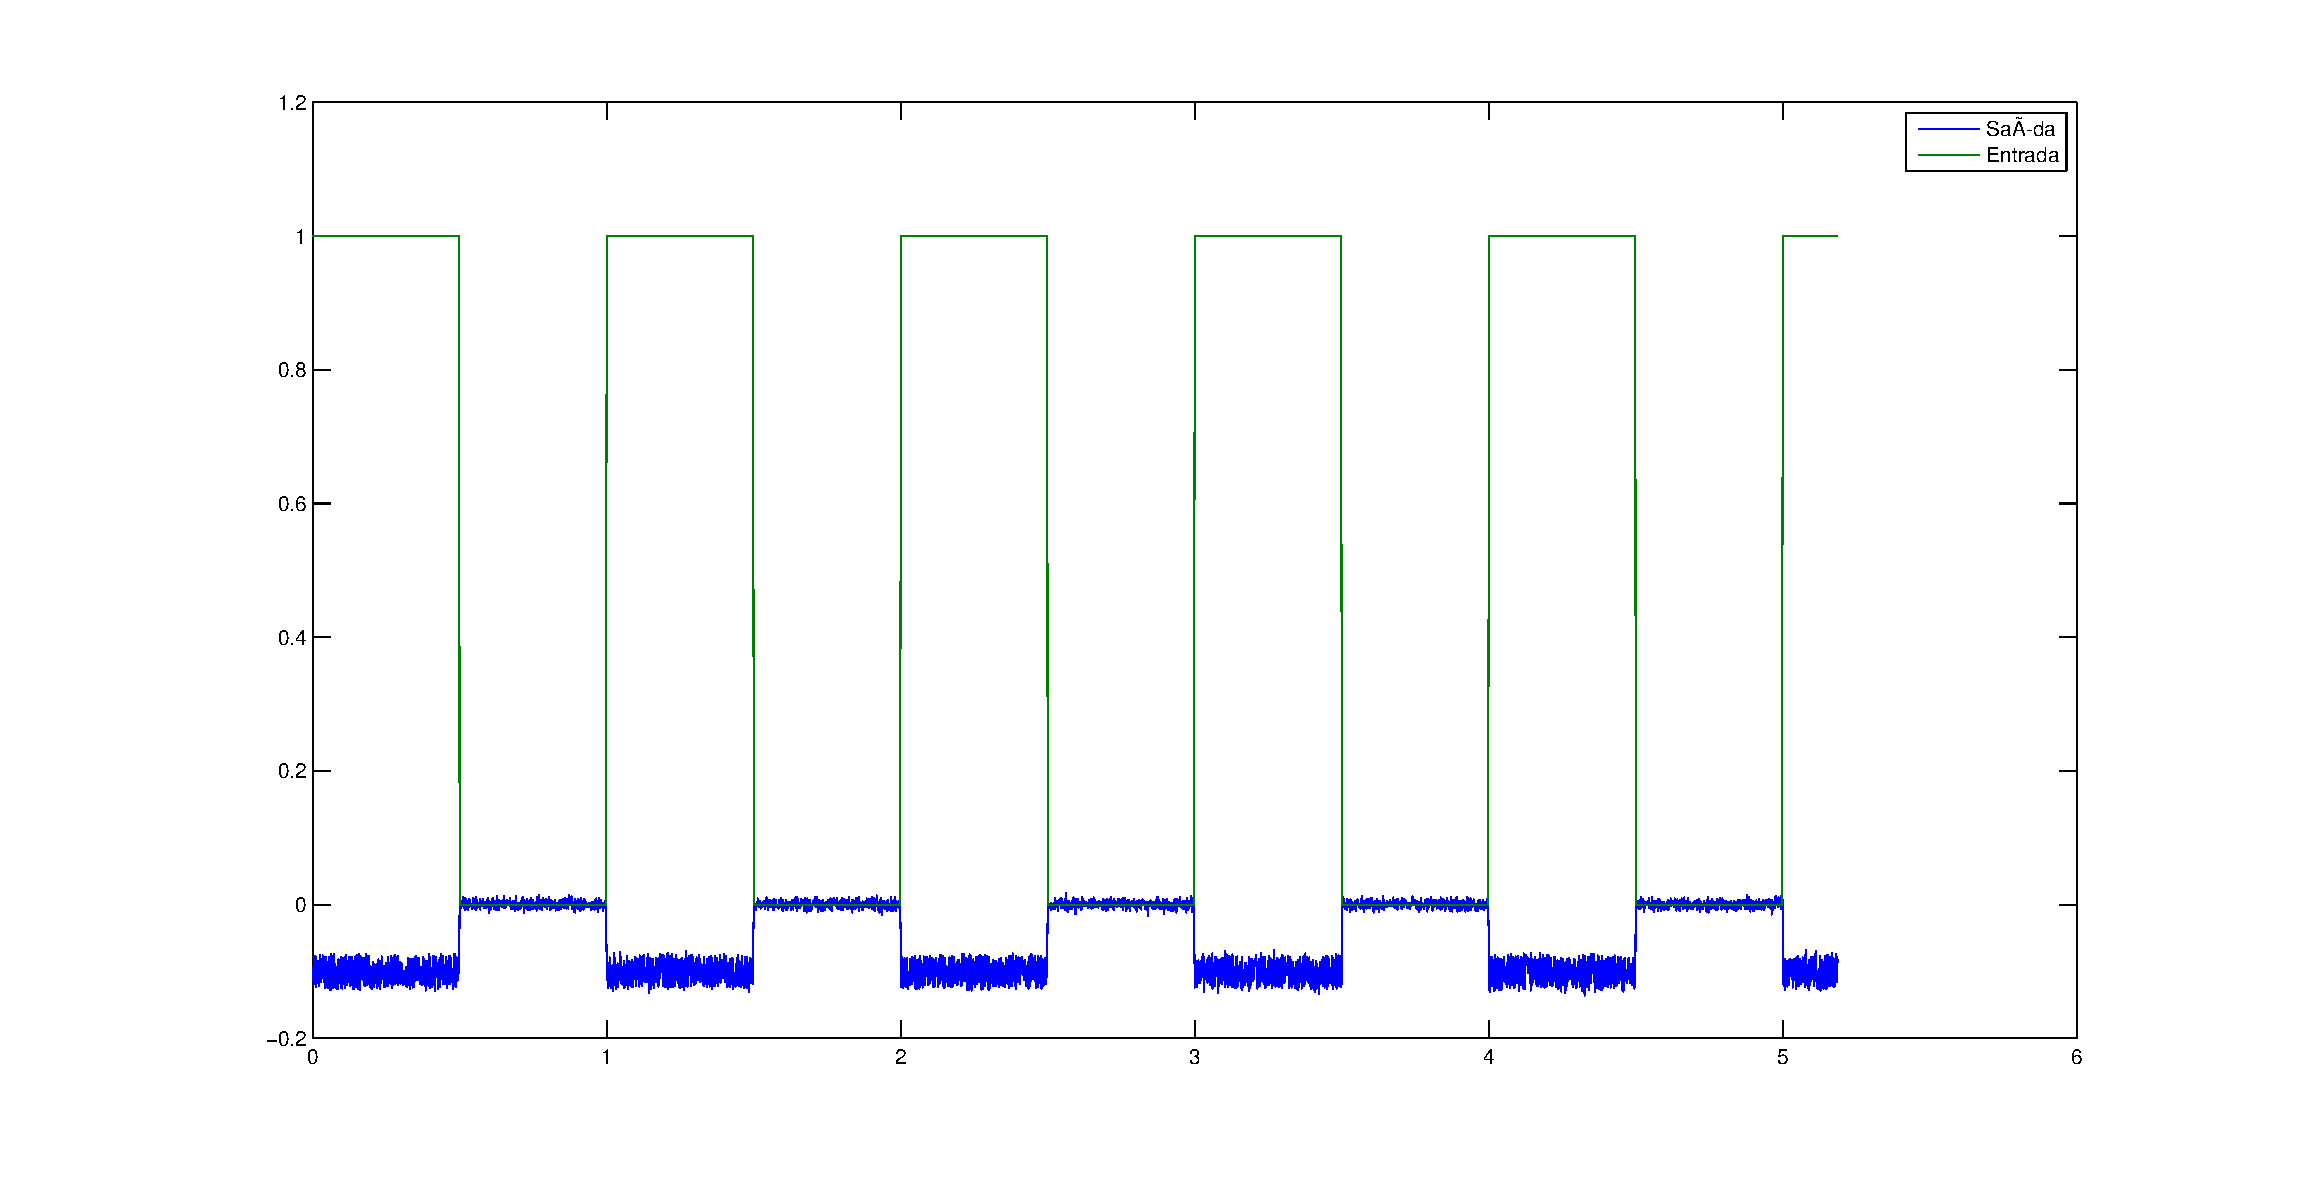
\includegraphics[width=\linewidth]{saida1}
	\caption{Medição da saída do primeiro estágio da planta}
	\label{fig:saida1}
\end{figure}
Conforme o roteiro \cite{bb:roteiro} sabemos que esse estágio trata-se de um ganho proporcional.
Analisamos então a razão entre saída e entrada, de maneira a determinar o ganho. Para isso, descartamos os pontos em que a entrada era zero e filtramos o sinal para diminuir o efeito de ruídos através tirando a média do sinal obtido (que deveria ser constante).
Com isso chegamos na função de transferência:
\begin{equation}
	\label{eq:g1}
	G_1(s) = -0.1005
\end{equation}
Que é bastante próxima do valor $0.1$ obtido no pré relatório.

\subsection{2$^o$ Estágio}
A medida obtida para o segundo estágio pode ser vista na figura \ref{fig:saida2}.
\begin{figure}[H]
	\centering
	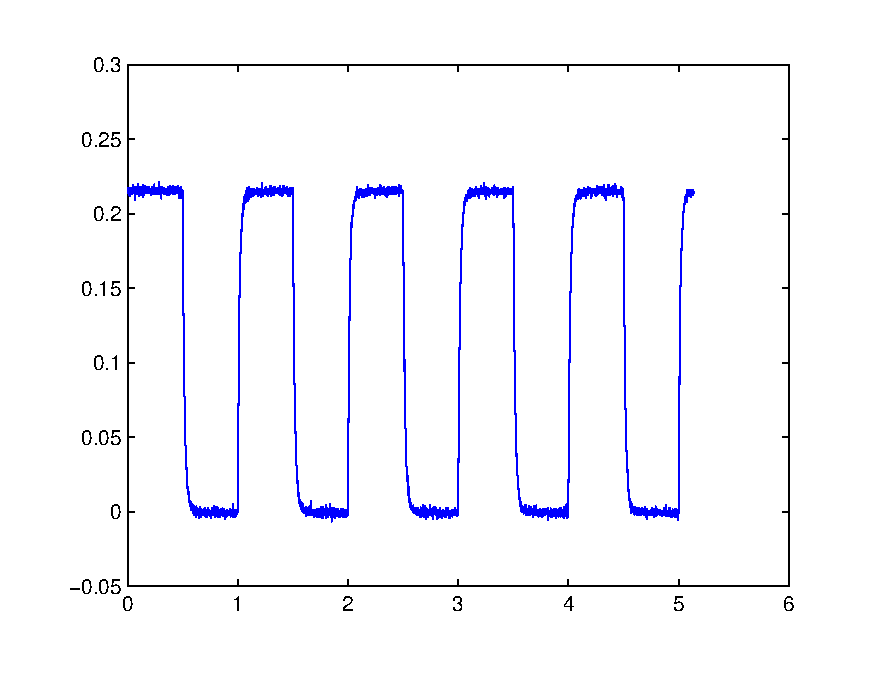
\includegraphics[width=\linewidth]{saida2}
	\caption{Medição da saída do segundo estágio da planta}
	\label{fig:saida2}
\end{figure}
Como podemos ver, essa sinal está ruidoso, logo utilizamos um filtro passa baixa de frequência de corte de $100Hz$ para prosseguir com a análise. A resposta em frequência para magnitude e fase desse filtro pode ser vista na figura \ref{fig:filtro} e o sinal filtrado pode é apresentado na figura \ref{fig:2filtrado}.
\begin{figure}[H]
	\centering
	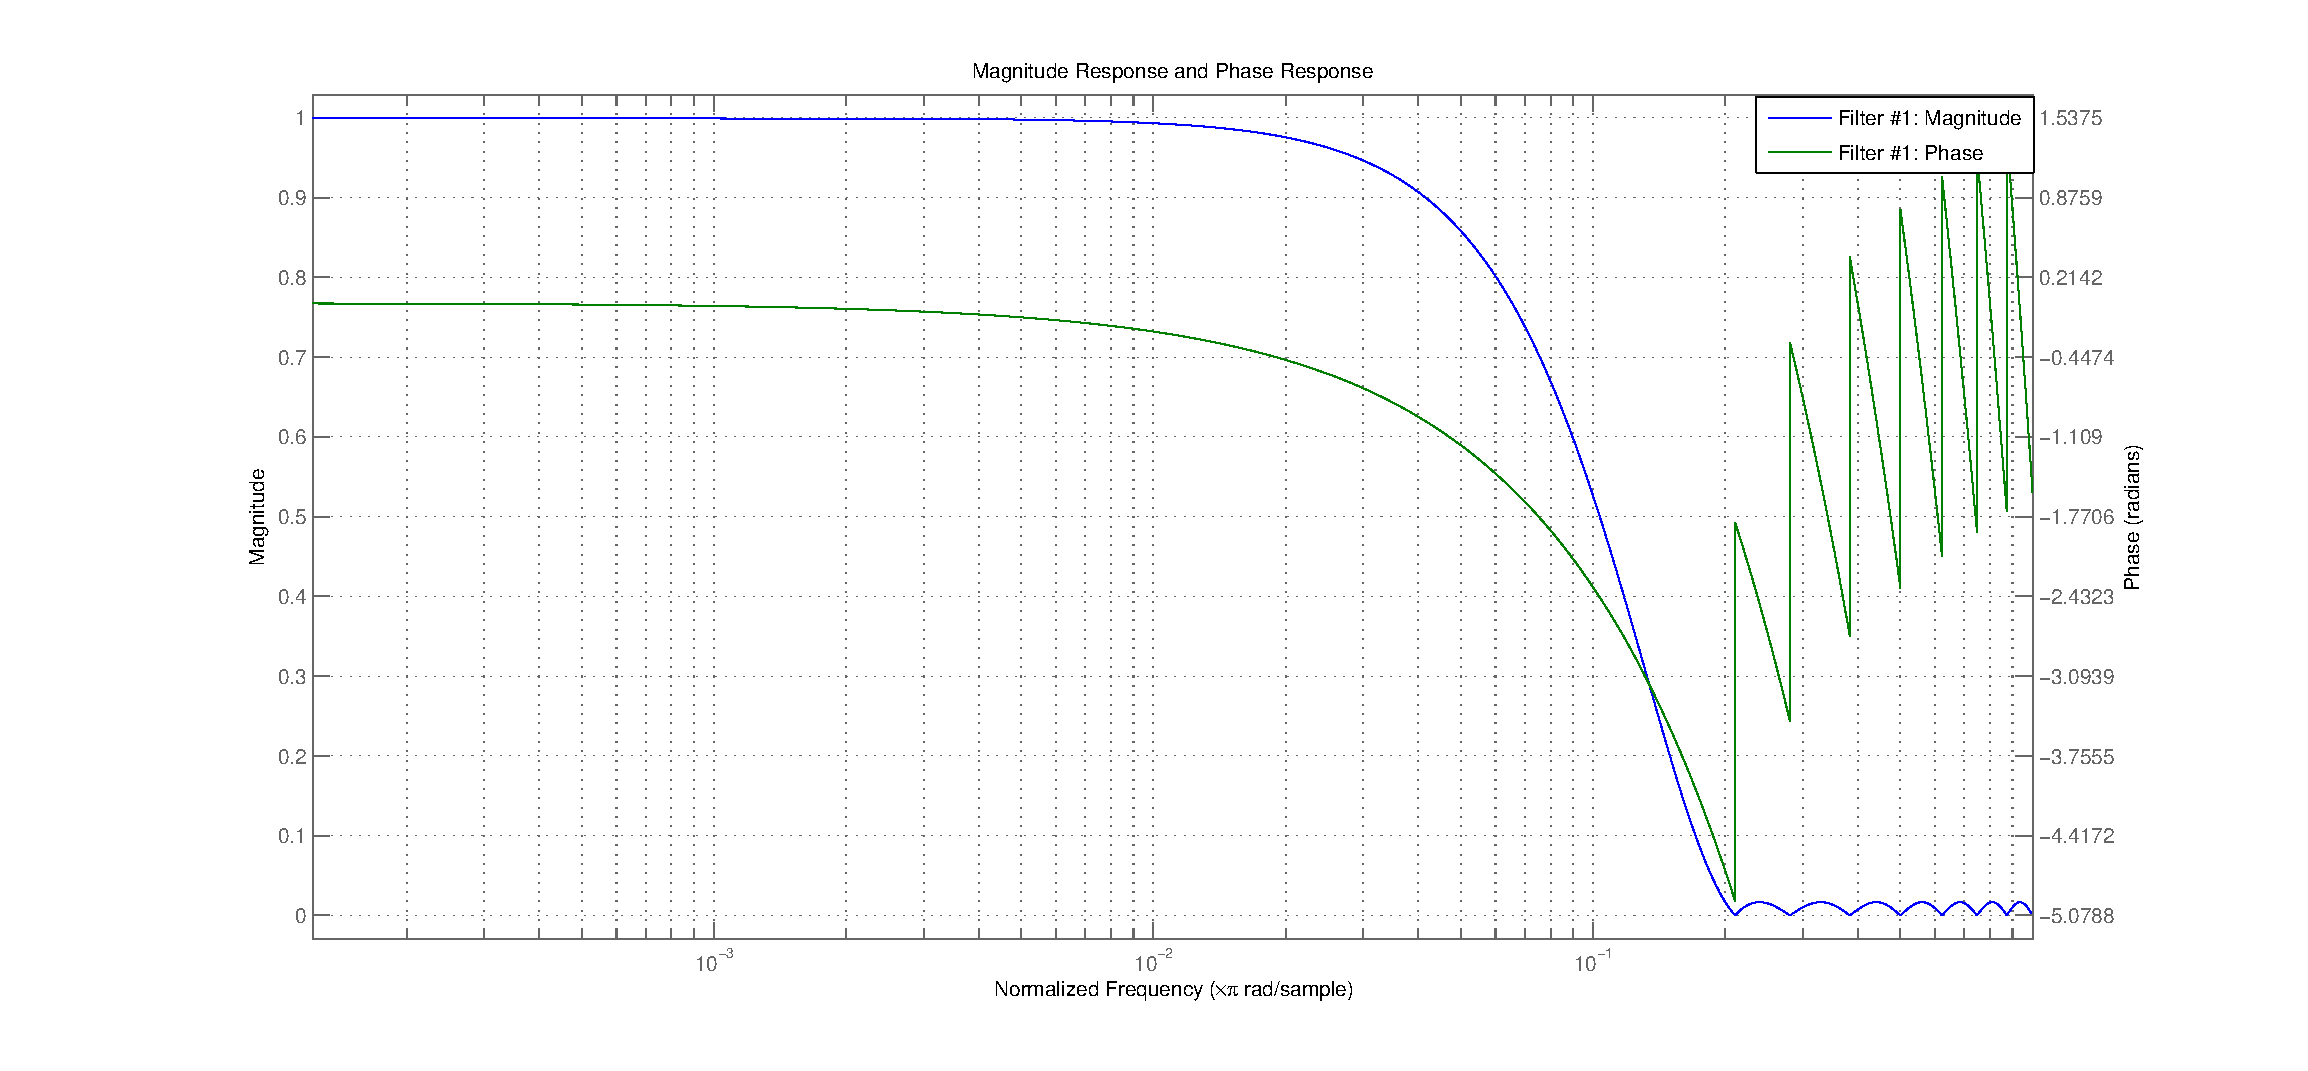
\includegraphics[width=\linewidth]{filtro}
	\caption{Resposta em frequência do filtro passa baixa}
	\label{fig:filtro}
\end{figure}
\begin{figure}[H]
	\centering
	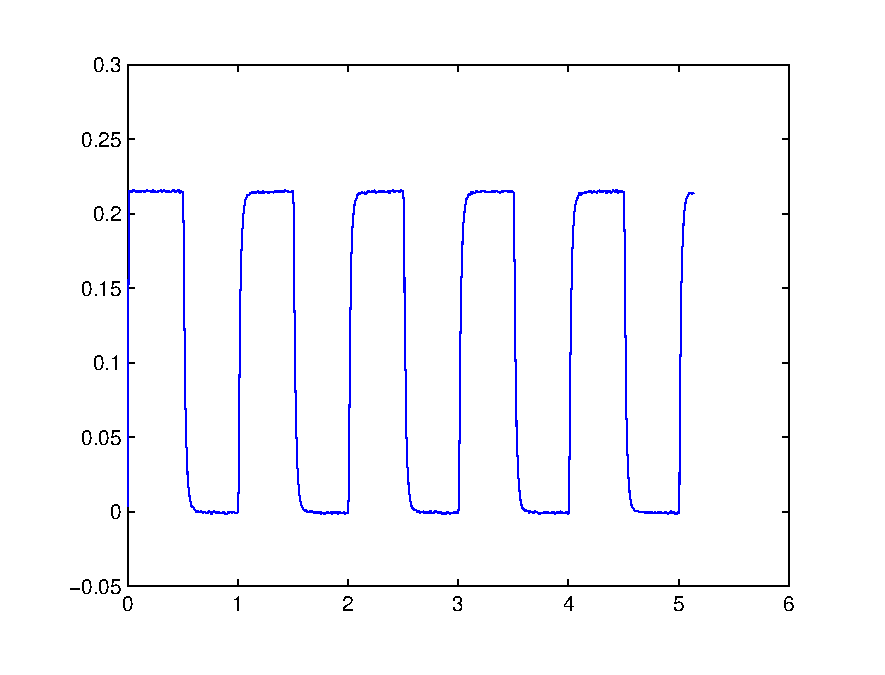
\includegraphics[width=\linewidth]{2filtrado}
	\caption{Medição filtrada da saída do segundo estágio da planta}
	\label{fig:2filtrado}
\end{figure}

Sabemos que a função de transferência desse estágio é da forma:
\begin{equation}
\label{eq:gs2}
G_2(s) = \frac{\kappa_2}{\tau_2 s + 1}
\end{equation}
Utilizamos o método apresentado no roteiro \cite{bb:roteiro} e encontramos o tempo de estabilização (para uma margem de $2\%$) $\tau_2 = 0.0210$ e o ganho $\kappa_2 = -2.1508$, conforme podemos ver na figura \ref{fig:2settling}. Esses valores também estão bem próximos dos calculados no pré relatório ($\kappa_2 = -2.2$ e $\tau_2 = 0.22$).
\begin{figure}[H]
	\centering
	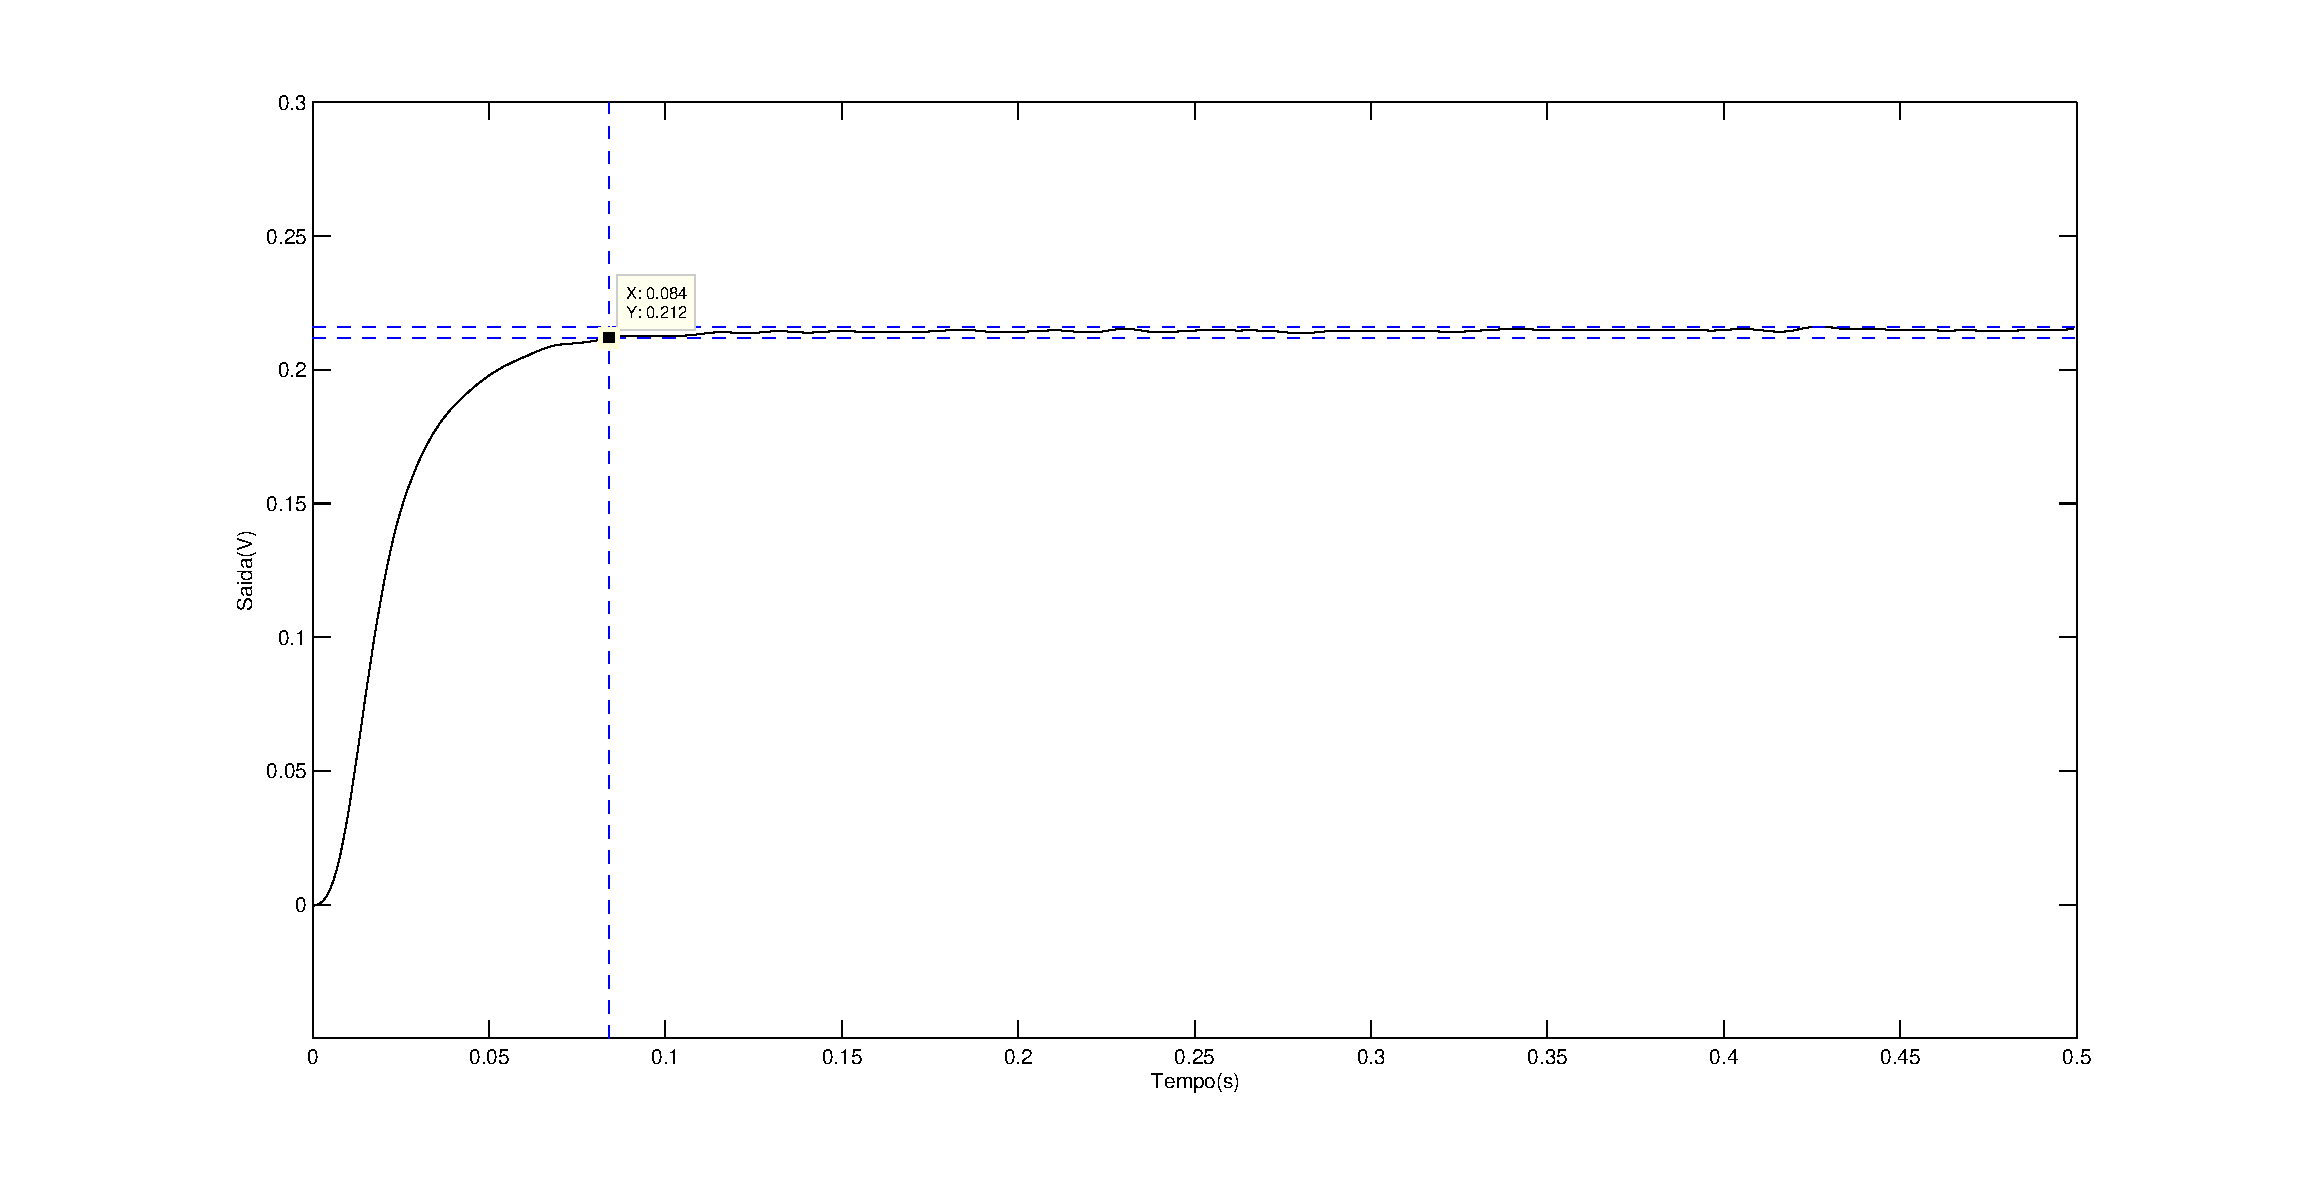
\includegraphics[width=\linewidth]{2settling}
	\caption{Tempo de estabilização para saída do estágio 2}
	\label{fig:2settling}
\end{figure}
Enfim, a função de transferência do estágio dois pode ser escrita como:
\begin{equation}
\label{eq:g2}
G_2(s) = \frac{-2.1508}{0.0210 s + 1}
\end{equation}

\subsection{3$^o$ Estágio}
A medida obtida para o terceiro estágio pode ser vista na figura \ref{fig:saida3} juntamente com o sinal filtrado.
\begin{figure}[H]
	\centering
	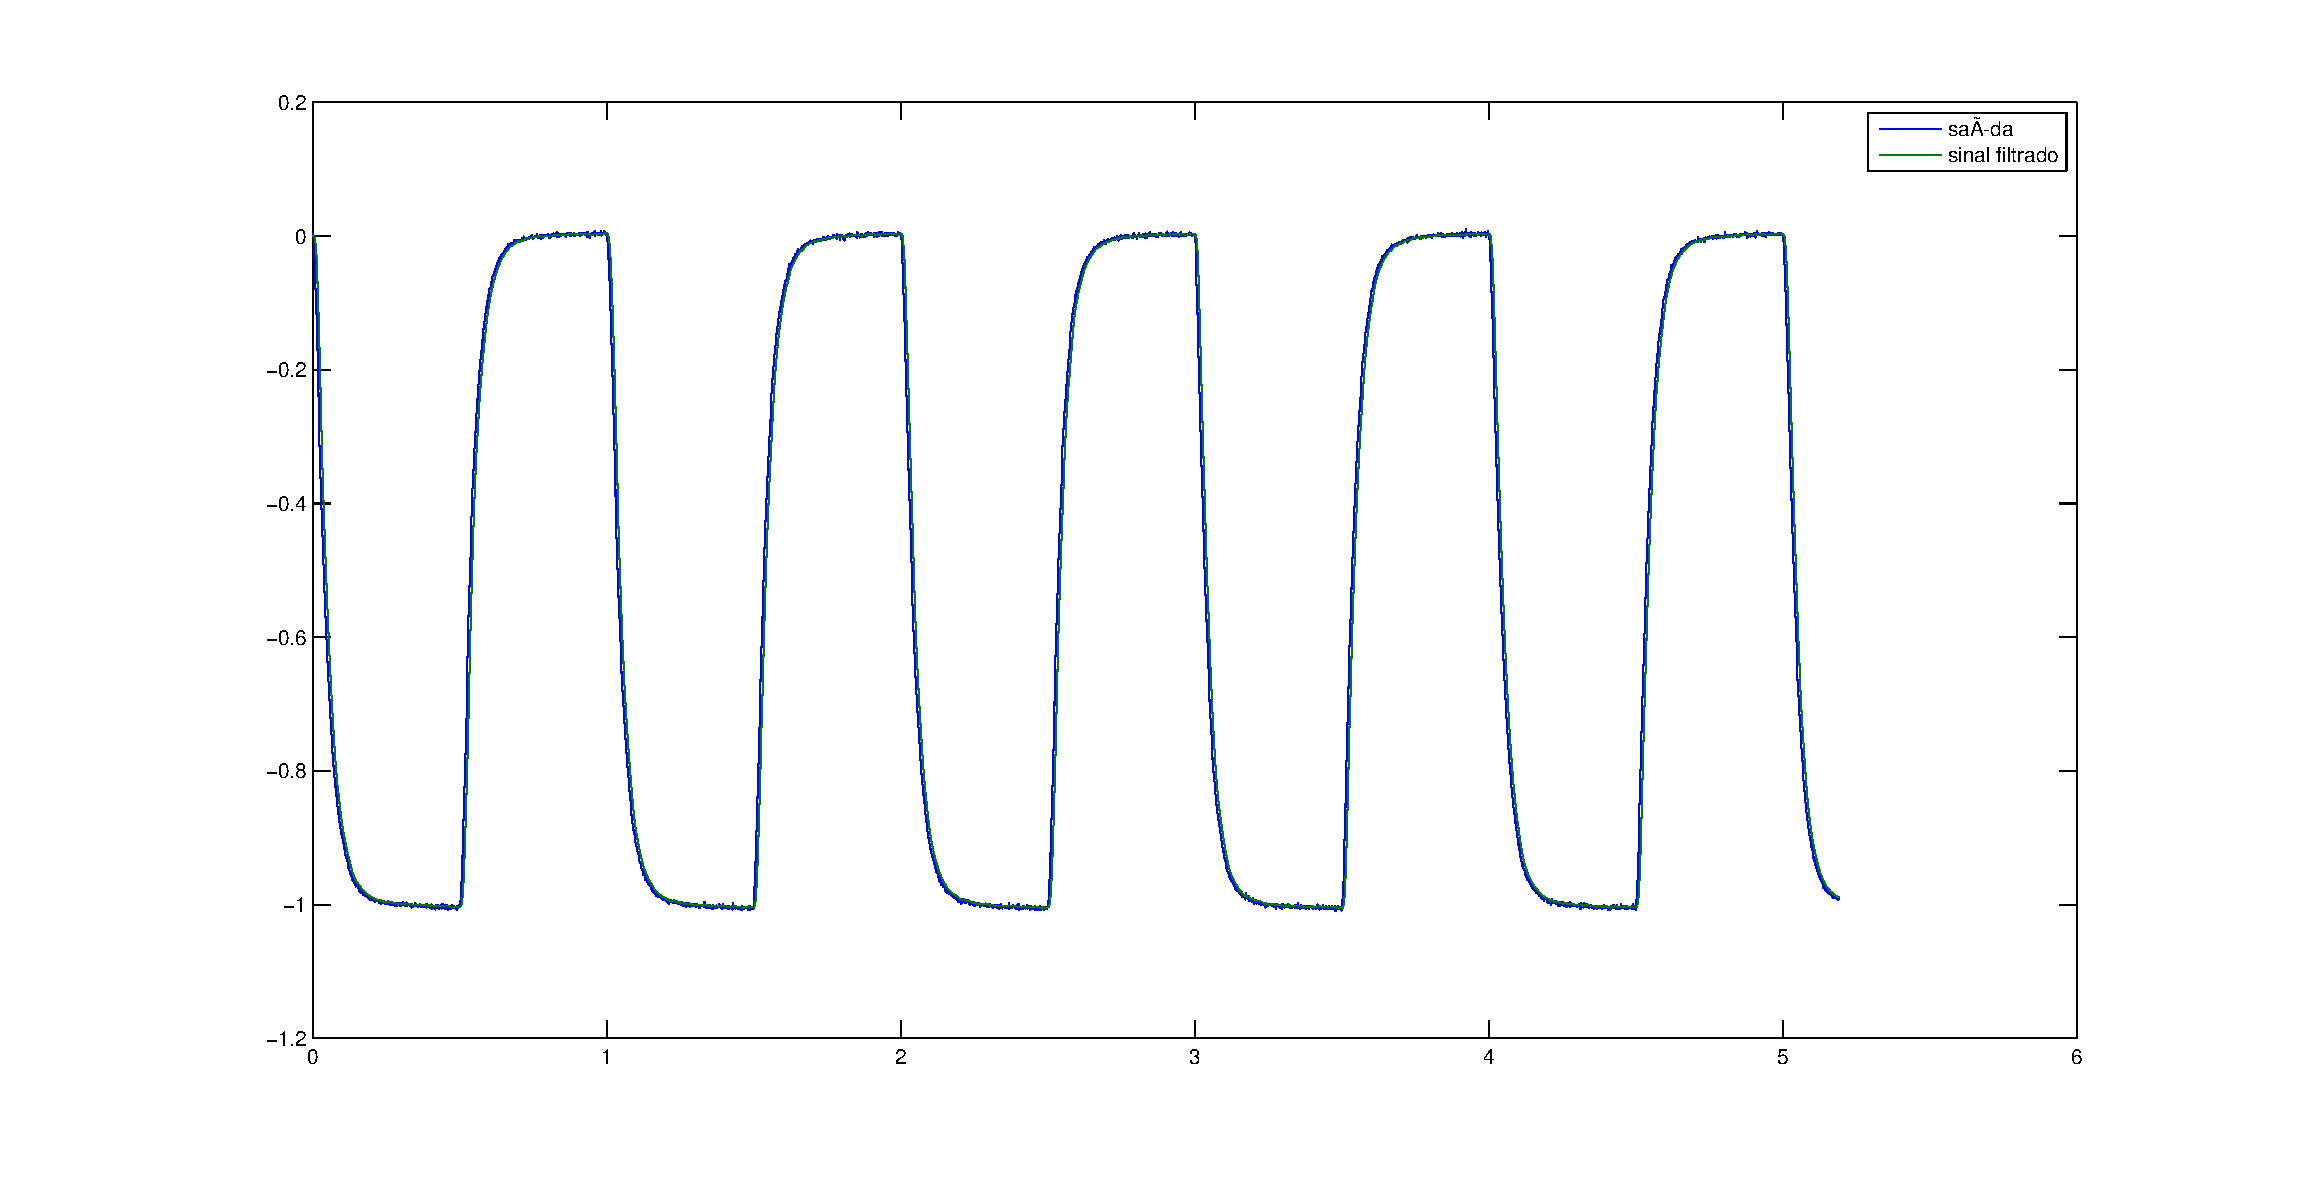
\includegraphics[width=\linewidth]{saida3}
	\caption{Medição e sinal filtrado da saída do terceiro estágio da planta}
	\label{fig:saida3}
\end{figure}
Utilizamos o método descrito no roteiro \cite{bb:roteiro} para encontrar os parâmetros da função de transferência desse estágio, que deve ser da forma:
\begin{equation}
\label{eq:gs3}
G_3(s) = \frac{\kappa_3}{\tau_3 s + 1}
\end{equation}
Para isso escolhemos os pontos de tempo $\tau_2$ e $2*\tau_2$ que podem ser visto na figura \ref{fig:3seila} para determinar o valor de $\tau_3$ através das equações do slide e analisamos a amplitude do sinal após sua estabilização para determinar $\kappa_3$.
\begin{figure}[H]
	\centering
	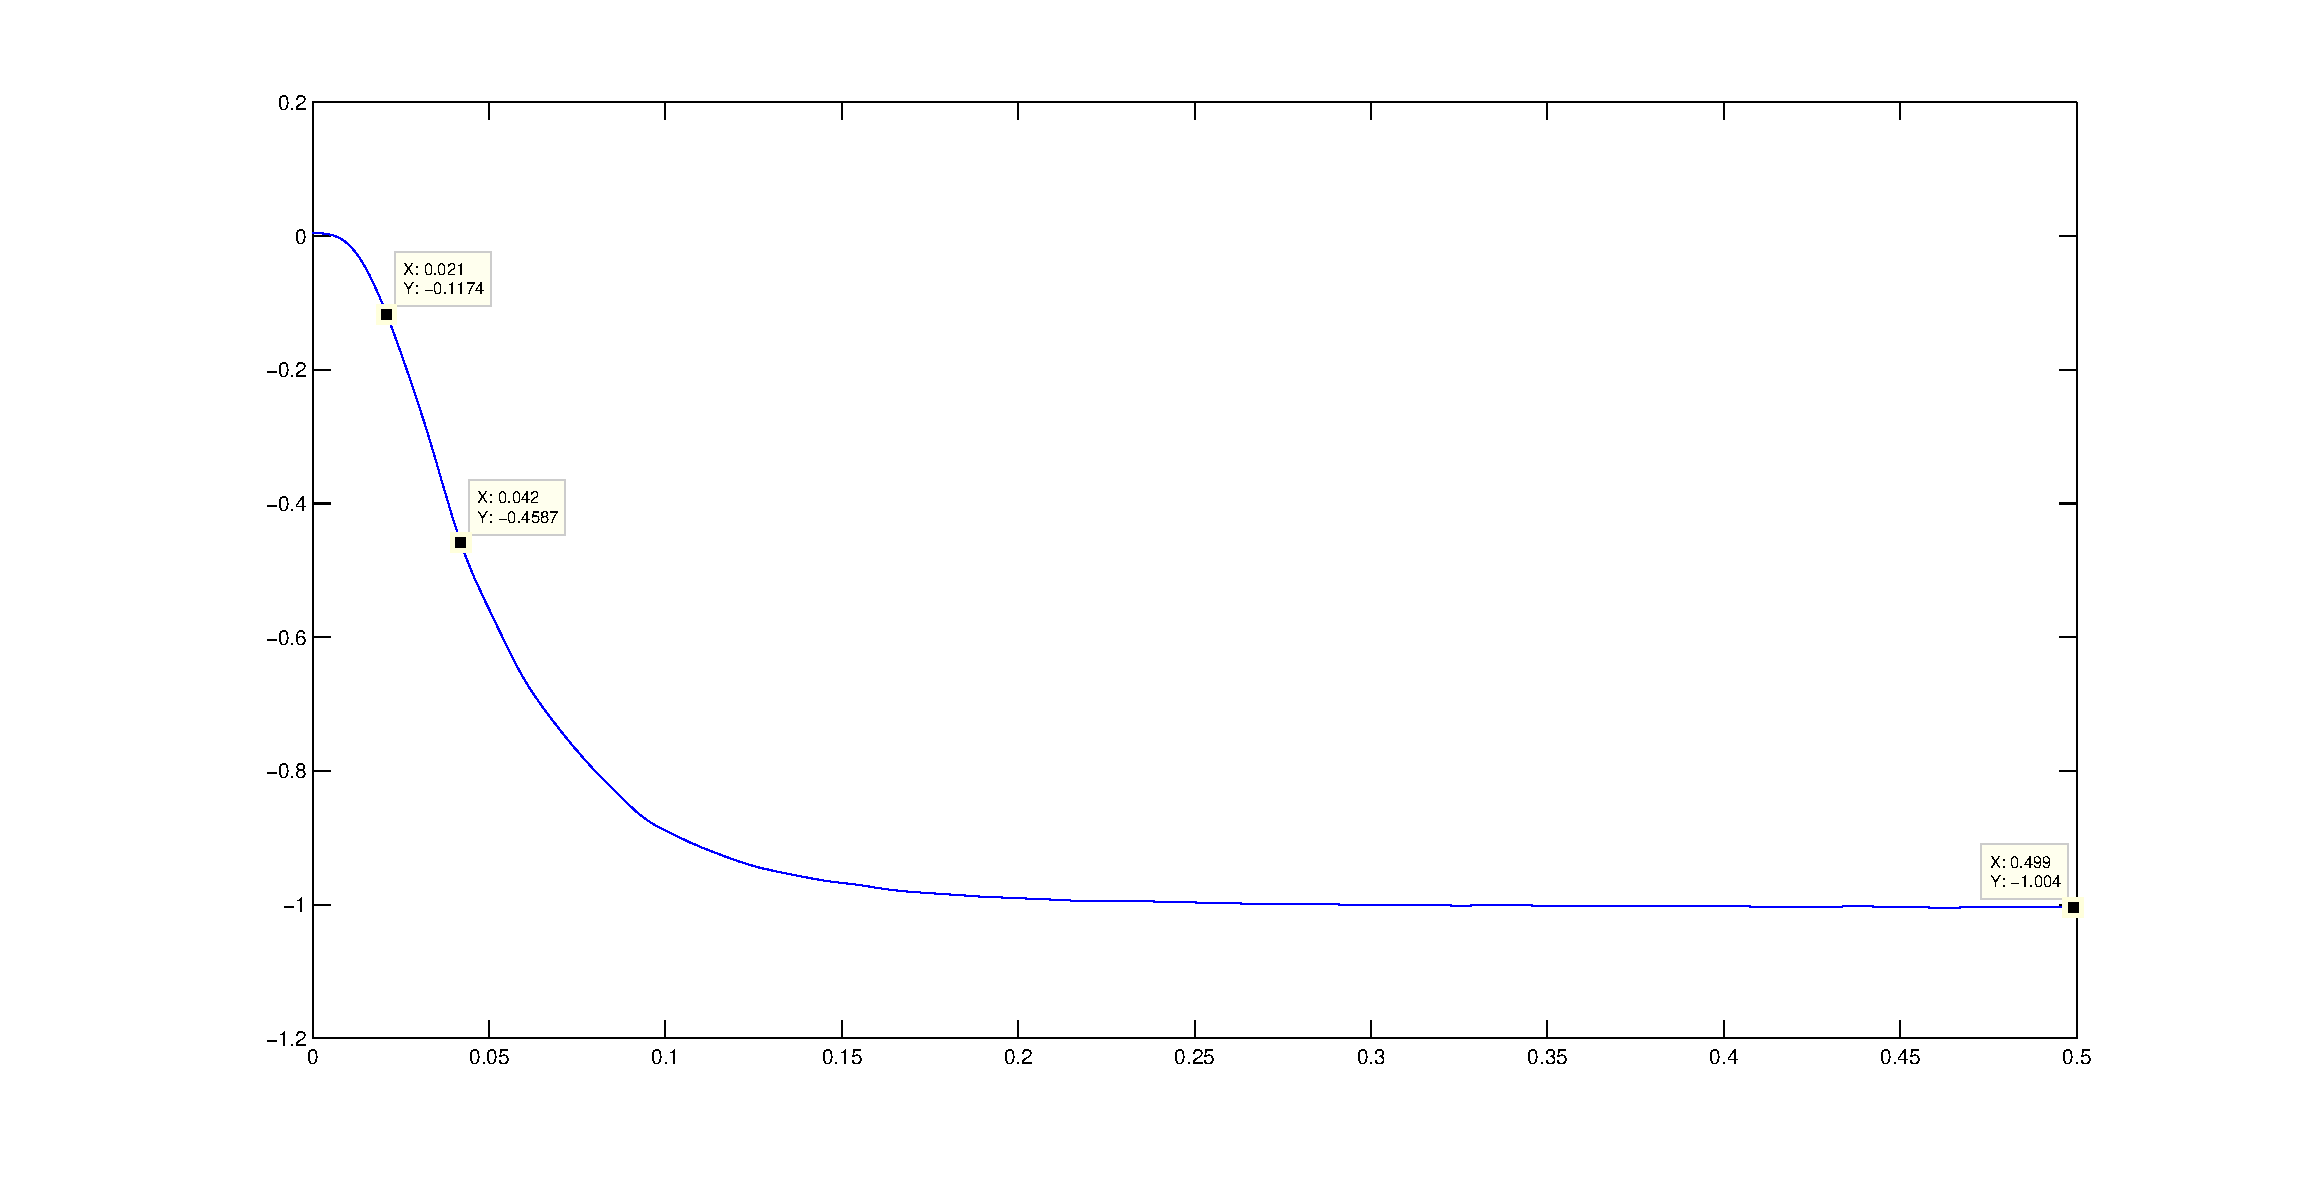
\includegraphics[width=\linewidth]{3seila}
	\caption{Resposta do terceiro estágio à um degrau com pontos de interesse}
	\label{fig:3seila}
\end{figure}
Encontramos então $\kappa_3 = -4.6448$ e $\tau_3 = 0.0244$, como podemos notar, o valor de $\kappa_3$ está bem próximo do valor de $-4.7$ encontrado no pré relatório, porém $\tau_3$ não. Acreditamos que as discrepâncias entre o resultado obtido e o valor de $0.47$ calculado previamente se devem as diferenças entre a implementação física e o circuito teórico analisado.
Enfim, obtivemos então:
\begin{equation}
\label{eq:g3}
G_3(s) = \frac{-4.6448}{0.0244 s + 1}
\end{equation}

\subsection{4$^o$ Estágio}
A medida obtida para o quarto estágio pode ser vista na figura \ref{fig:saida4} juntamente com o sinal filtrado.
\begin{figure}[H]
	\centering
	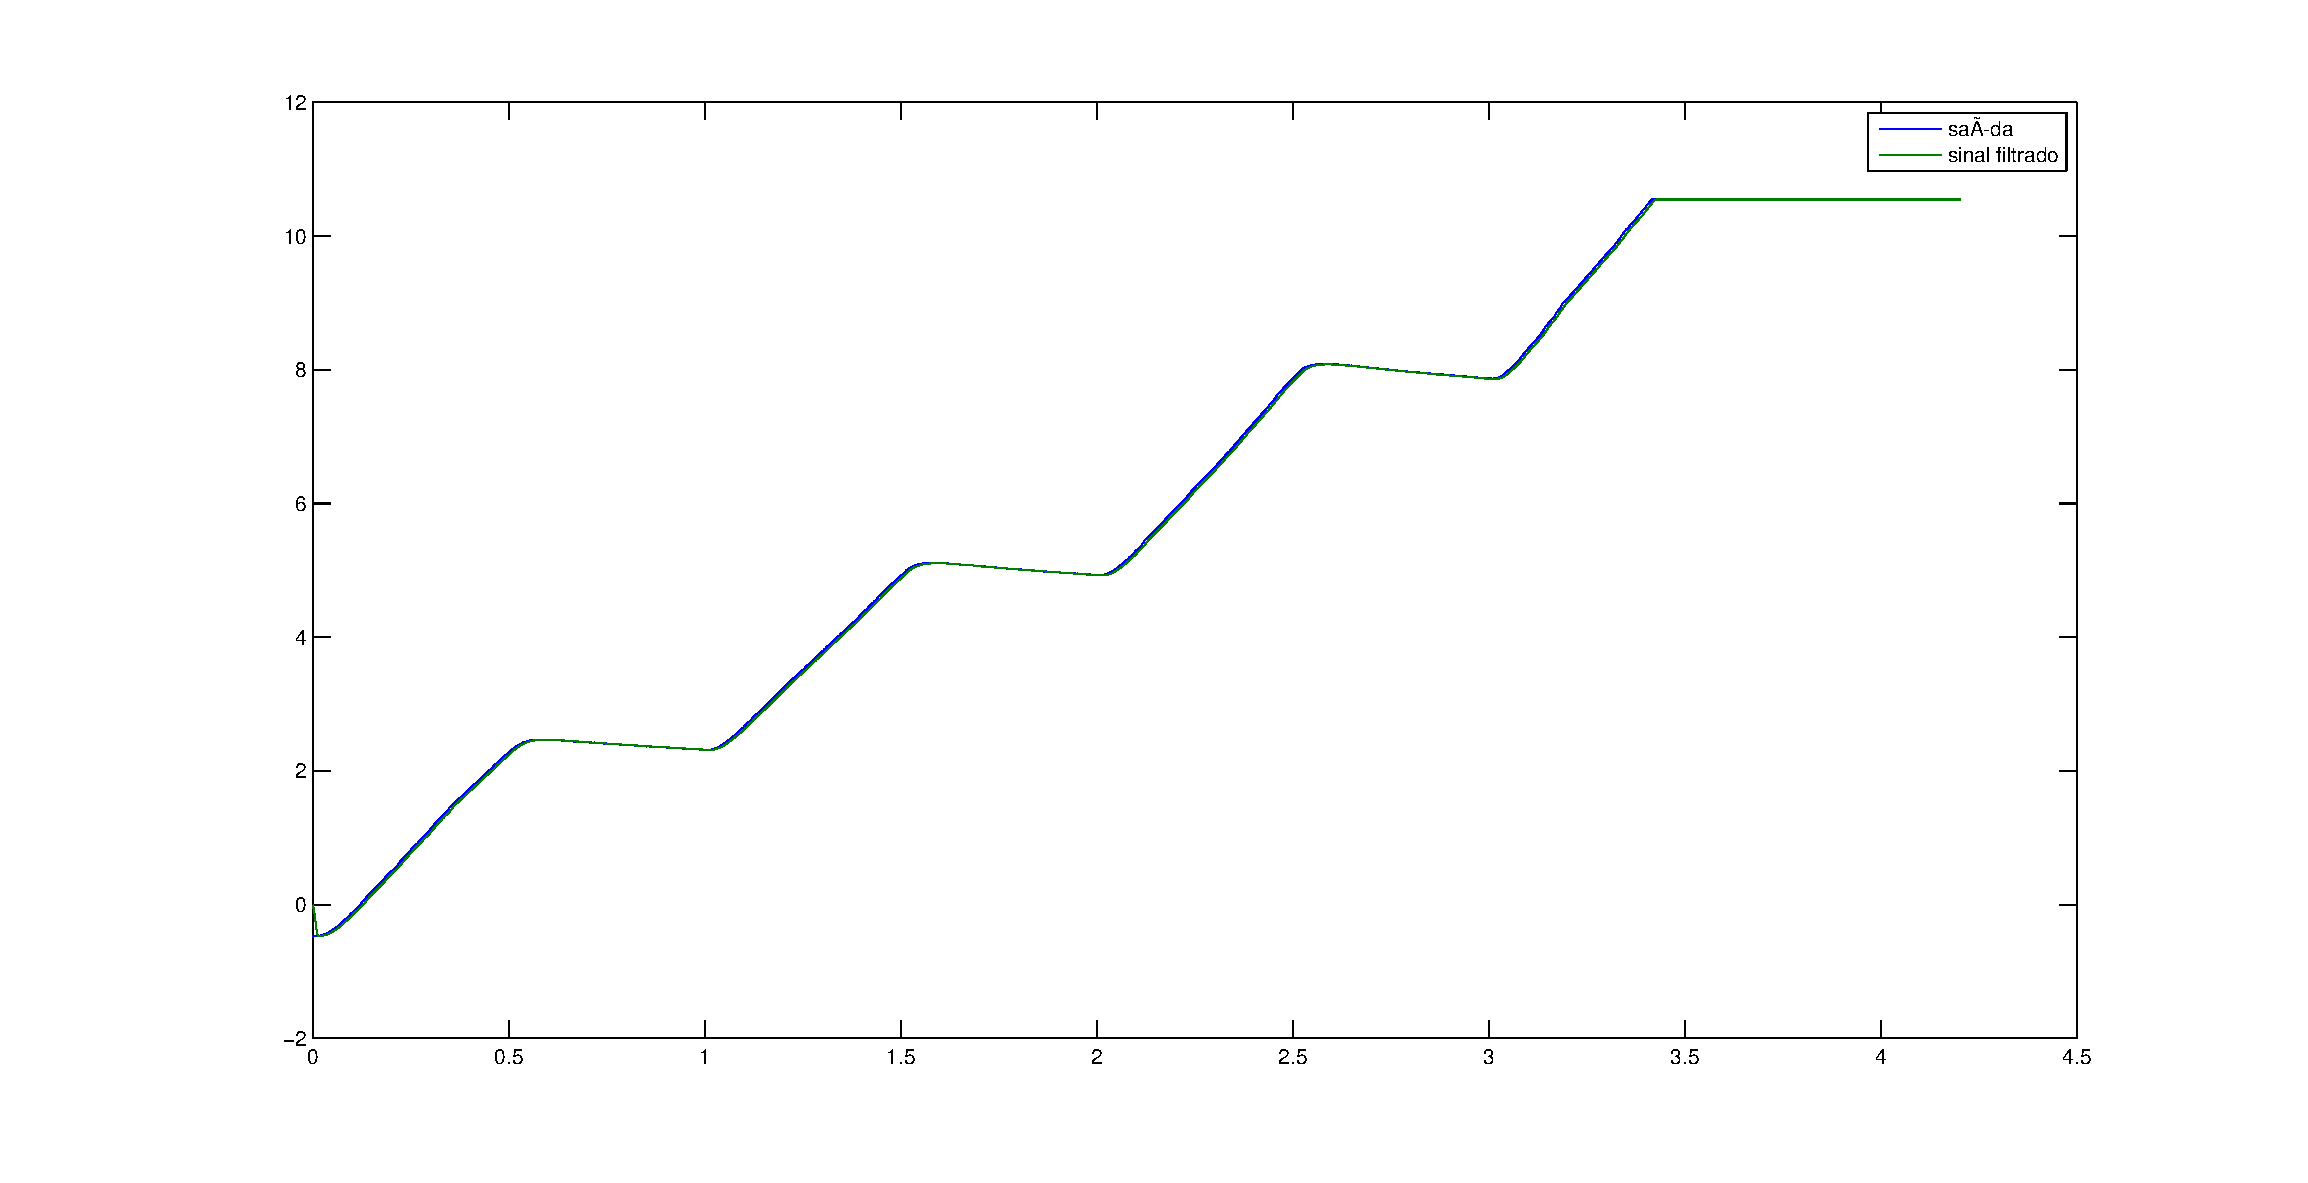
\includegraphics[width=\linewidth]{saida4}
	\caption{Medição e sinal filtrado da saída do quarto estágio da planta}
	\label{fig:saida4}
\end{figure}
Sabemos que esse estágio trata-se de um integrador, cuja função de transferência é do tipo:
\begin{equation}
\label{eq:gs4}
G_4(s) = \frac{\kappa_4}{s}
\end{equation}
Logo, para determinar o parâmetro $\kappa_4$ isolamos a resposta do sistema a um degrau e calculamos a inclinação da reta para $t >> \tau_3$, de maneira a observar somente a resposta à uma entrada constante com os pontos que podem ser vistos na figura \ref{fig:4seila}. 
\begin{figure}[H]
	\centering
	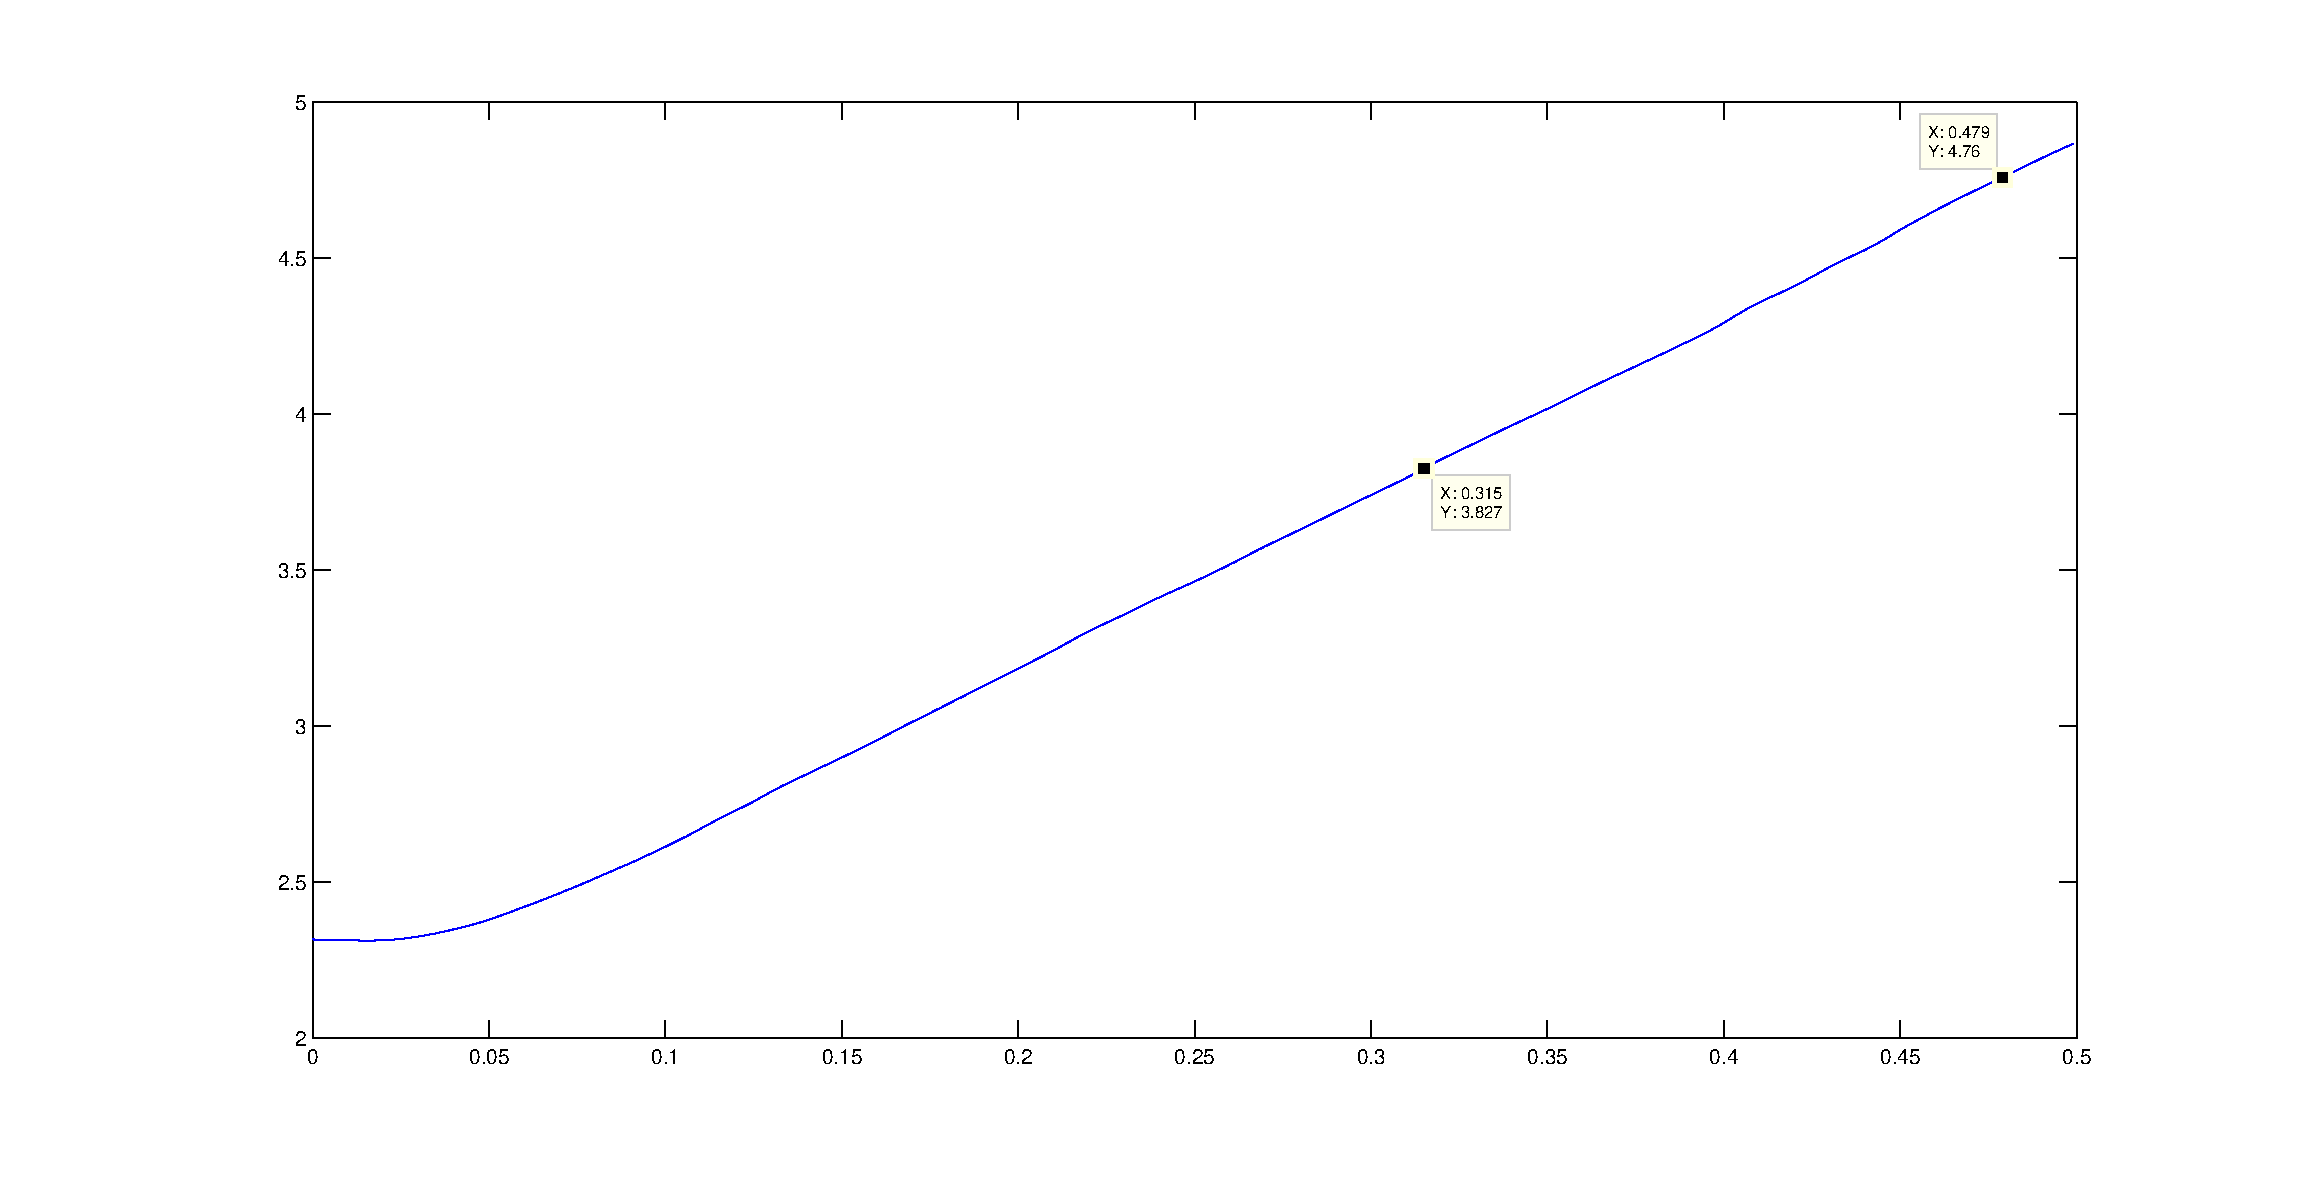
\includegraphics[width=\linewidth]{4seila}
	\caption{Resposta do quarto estágio à um degrau com pontos de interesse}
	\label{fig:4seila}
\end{figure}
Obtivemos o valor $\kappa_4 = -5.6700$ que é bem diferente do valor de $-10$ obtido no pré relatório, acreditamos que essa discrepância se deve também às diferenças entre o sistema físico e o teórico. A função de transferência do estágio quatro é então:
\begin{equation}
\label{eq:g4}
G_4(s) = \frac{-5.6700}{s}
\end{equation} 

\section{Conclusão}
Com esse experimento determinamos que nossa planta segue a função de transferência:
\begin{equation}
\label{eq:gs}
G(s) = \frac{5.693}{0.0005134 s^3 + 0.04545 s^2 + s}
\end{equation} 
Essa função é diferente da obtida no pré relatório principalmente devido aos valores $\tau_3$ e $\kappa_4$, porém podemos observar que ela é condizente com as medidas obtidas através da simulação das respostas de cada estágio à mesma entrada do sistema físico que podem ser observados nas figuras \ref{fig:sim1}, \ref{fig:sim2}, \ref{fig:sim3} e \ref{fig:sim4}.
\begin{figure}[H]
	\centering
	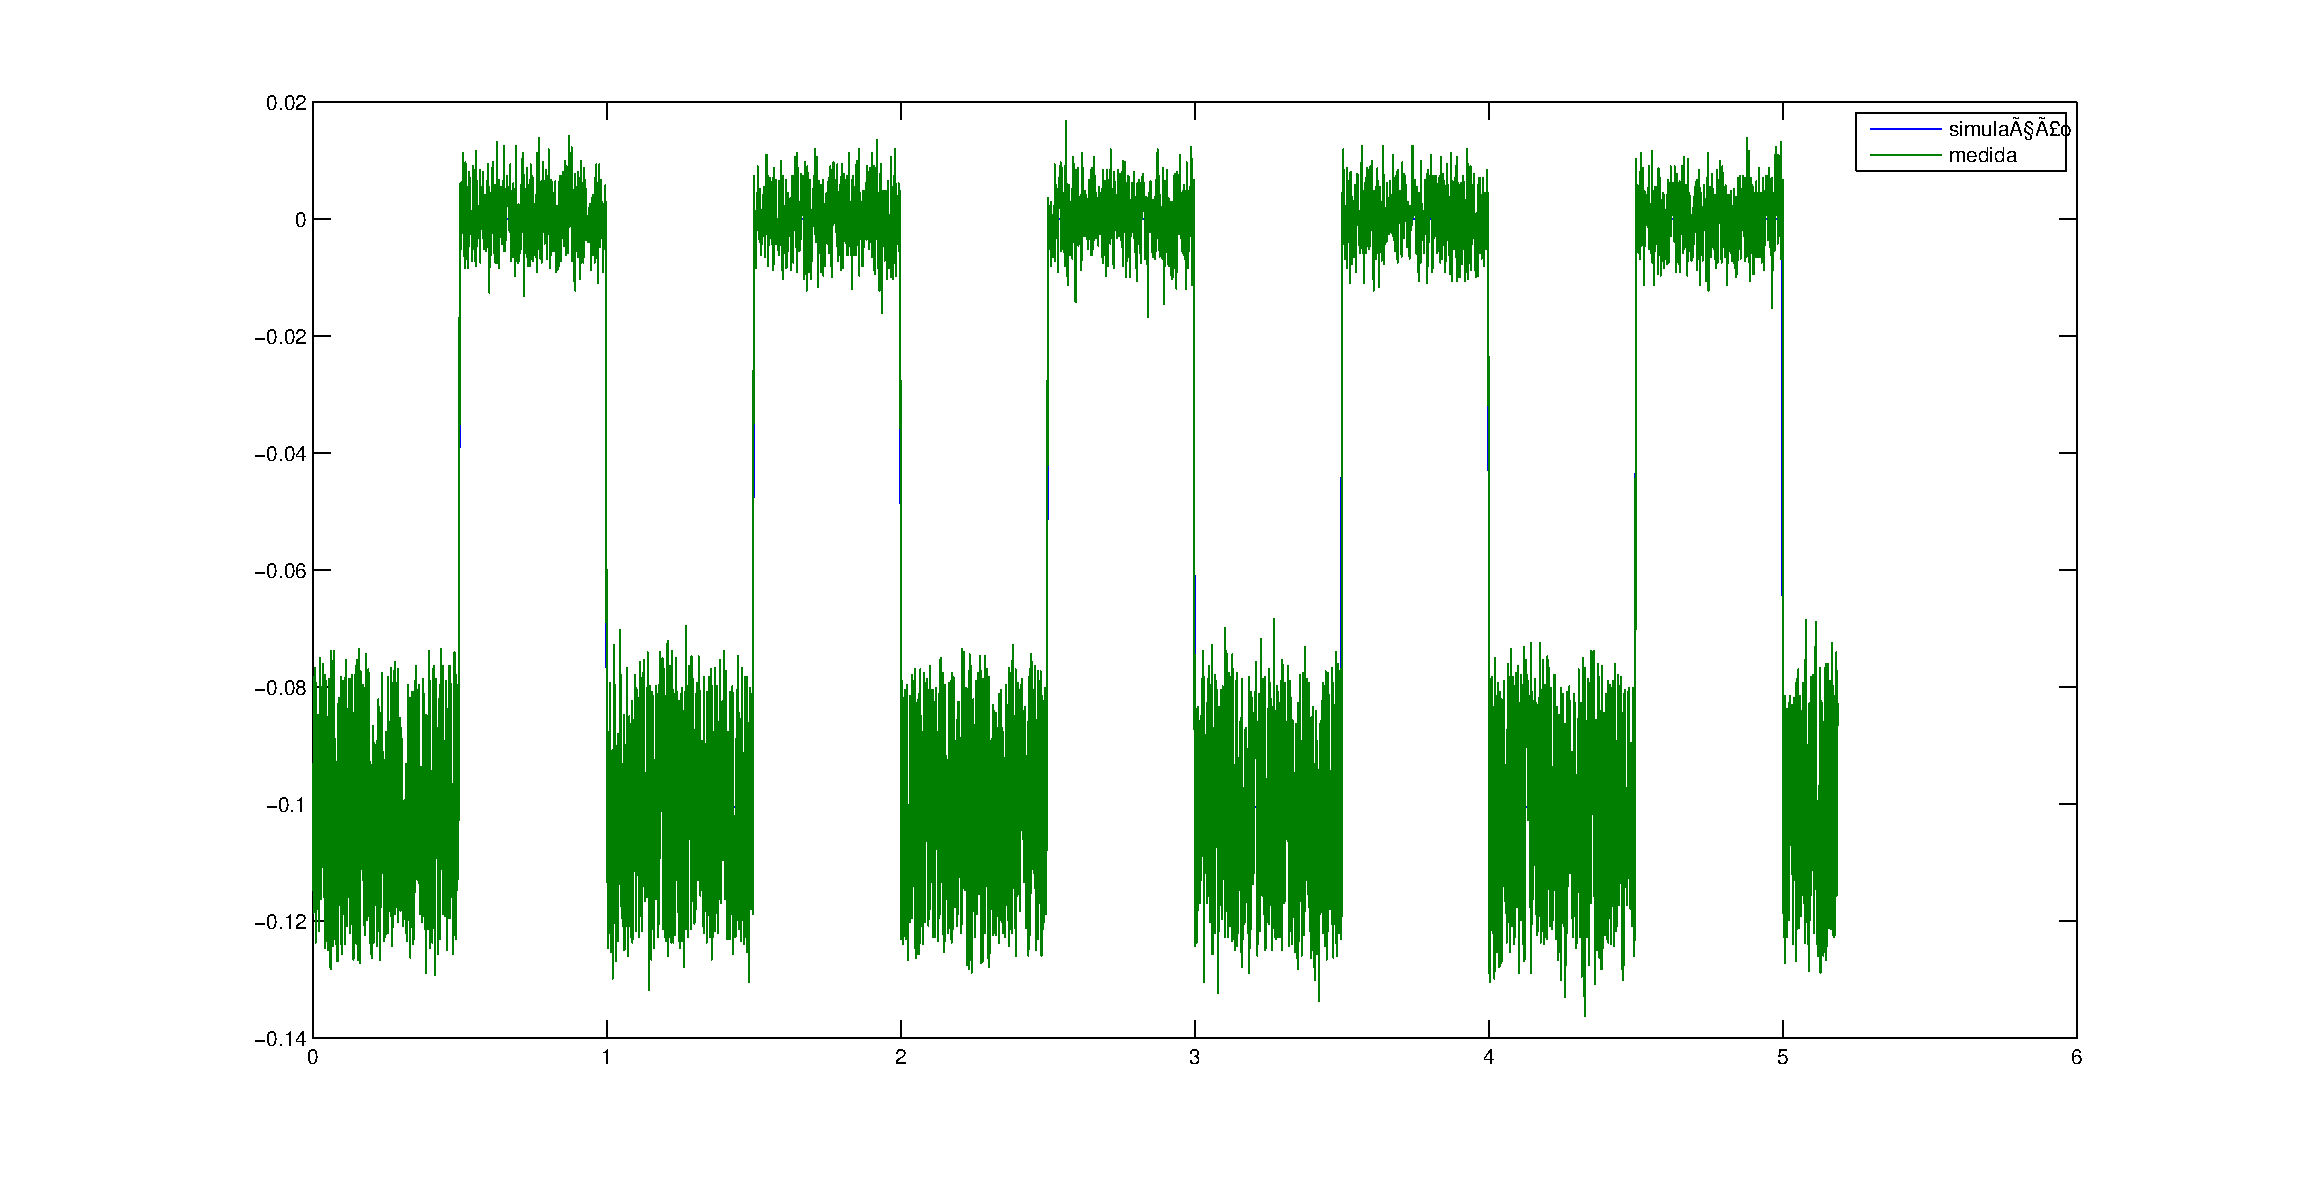
\includegraphics[width=0.8\linewidth]{sim1}
	\caption{Resposta do primeiro estágio à uma onda quadrada e simulação da mesma}
	\label{fig:sim1}
\end{figure}
\begin{figure}[H]
	\centering
	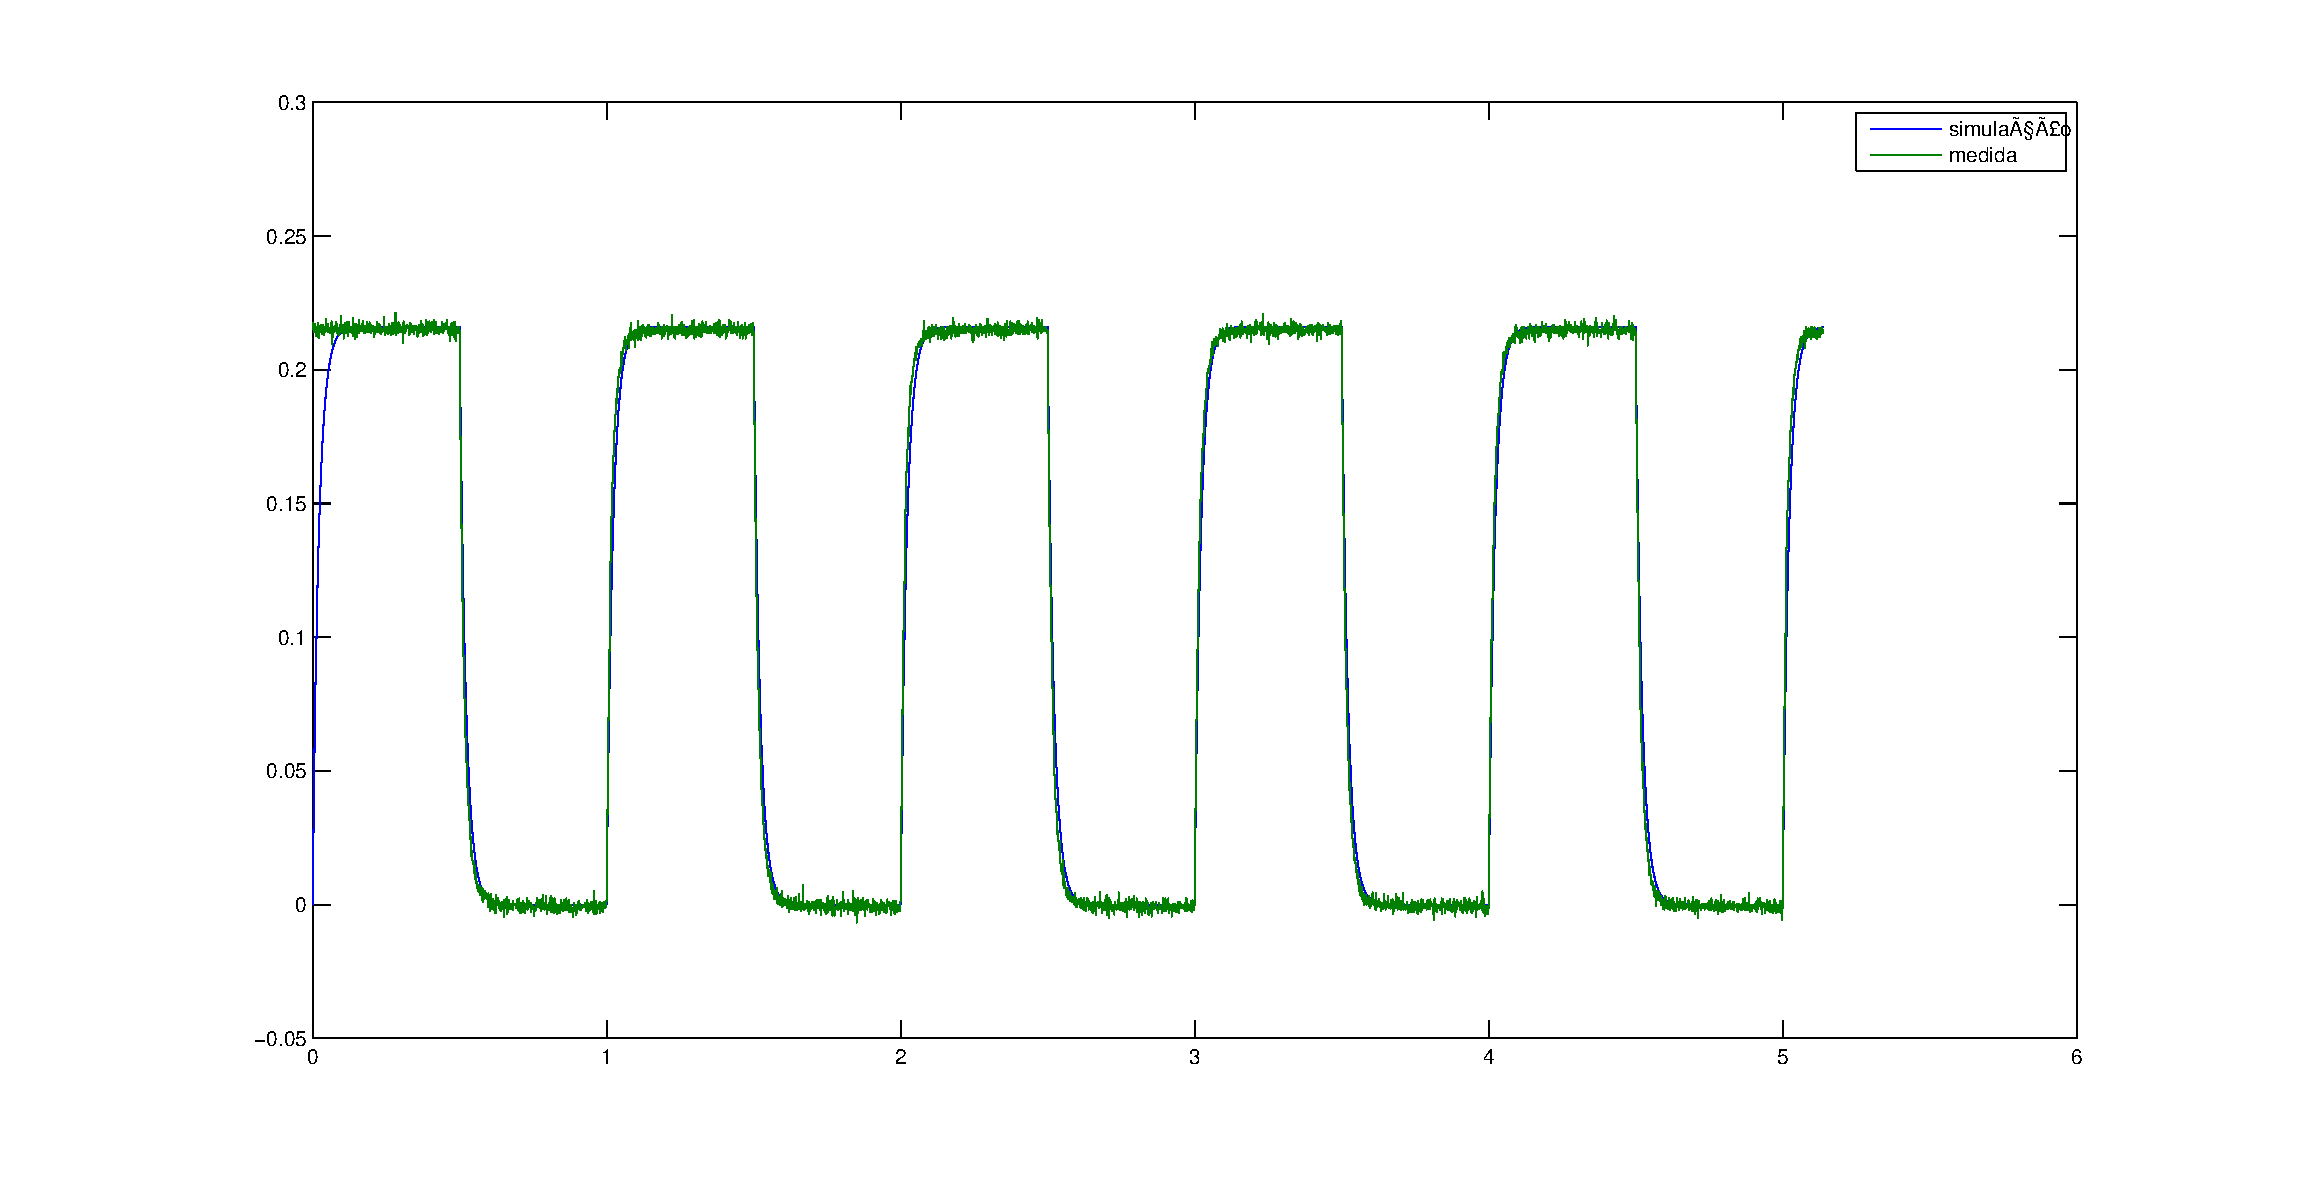
\includegraphics[width=0.8\linewidth]{sim2}
	\caption{Resposta do segundo estágio à uma onda quadrada e simulação da mesma}
	\label{fig:sim2}
\end{figure}
\begin{figure}[H]
	\centering
	\includegraphics[width=0.8\linewidth]{sim3}
	\caption{Resposta do terceiro estágio à uma onda quadrada e simulação da mesma}
	\label{fig:sim3}
\end{figure}
\begin{figure}[H]
	\centering
	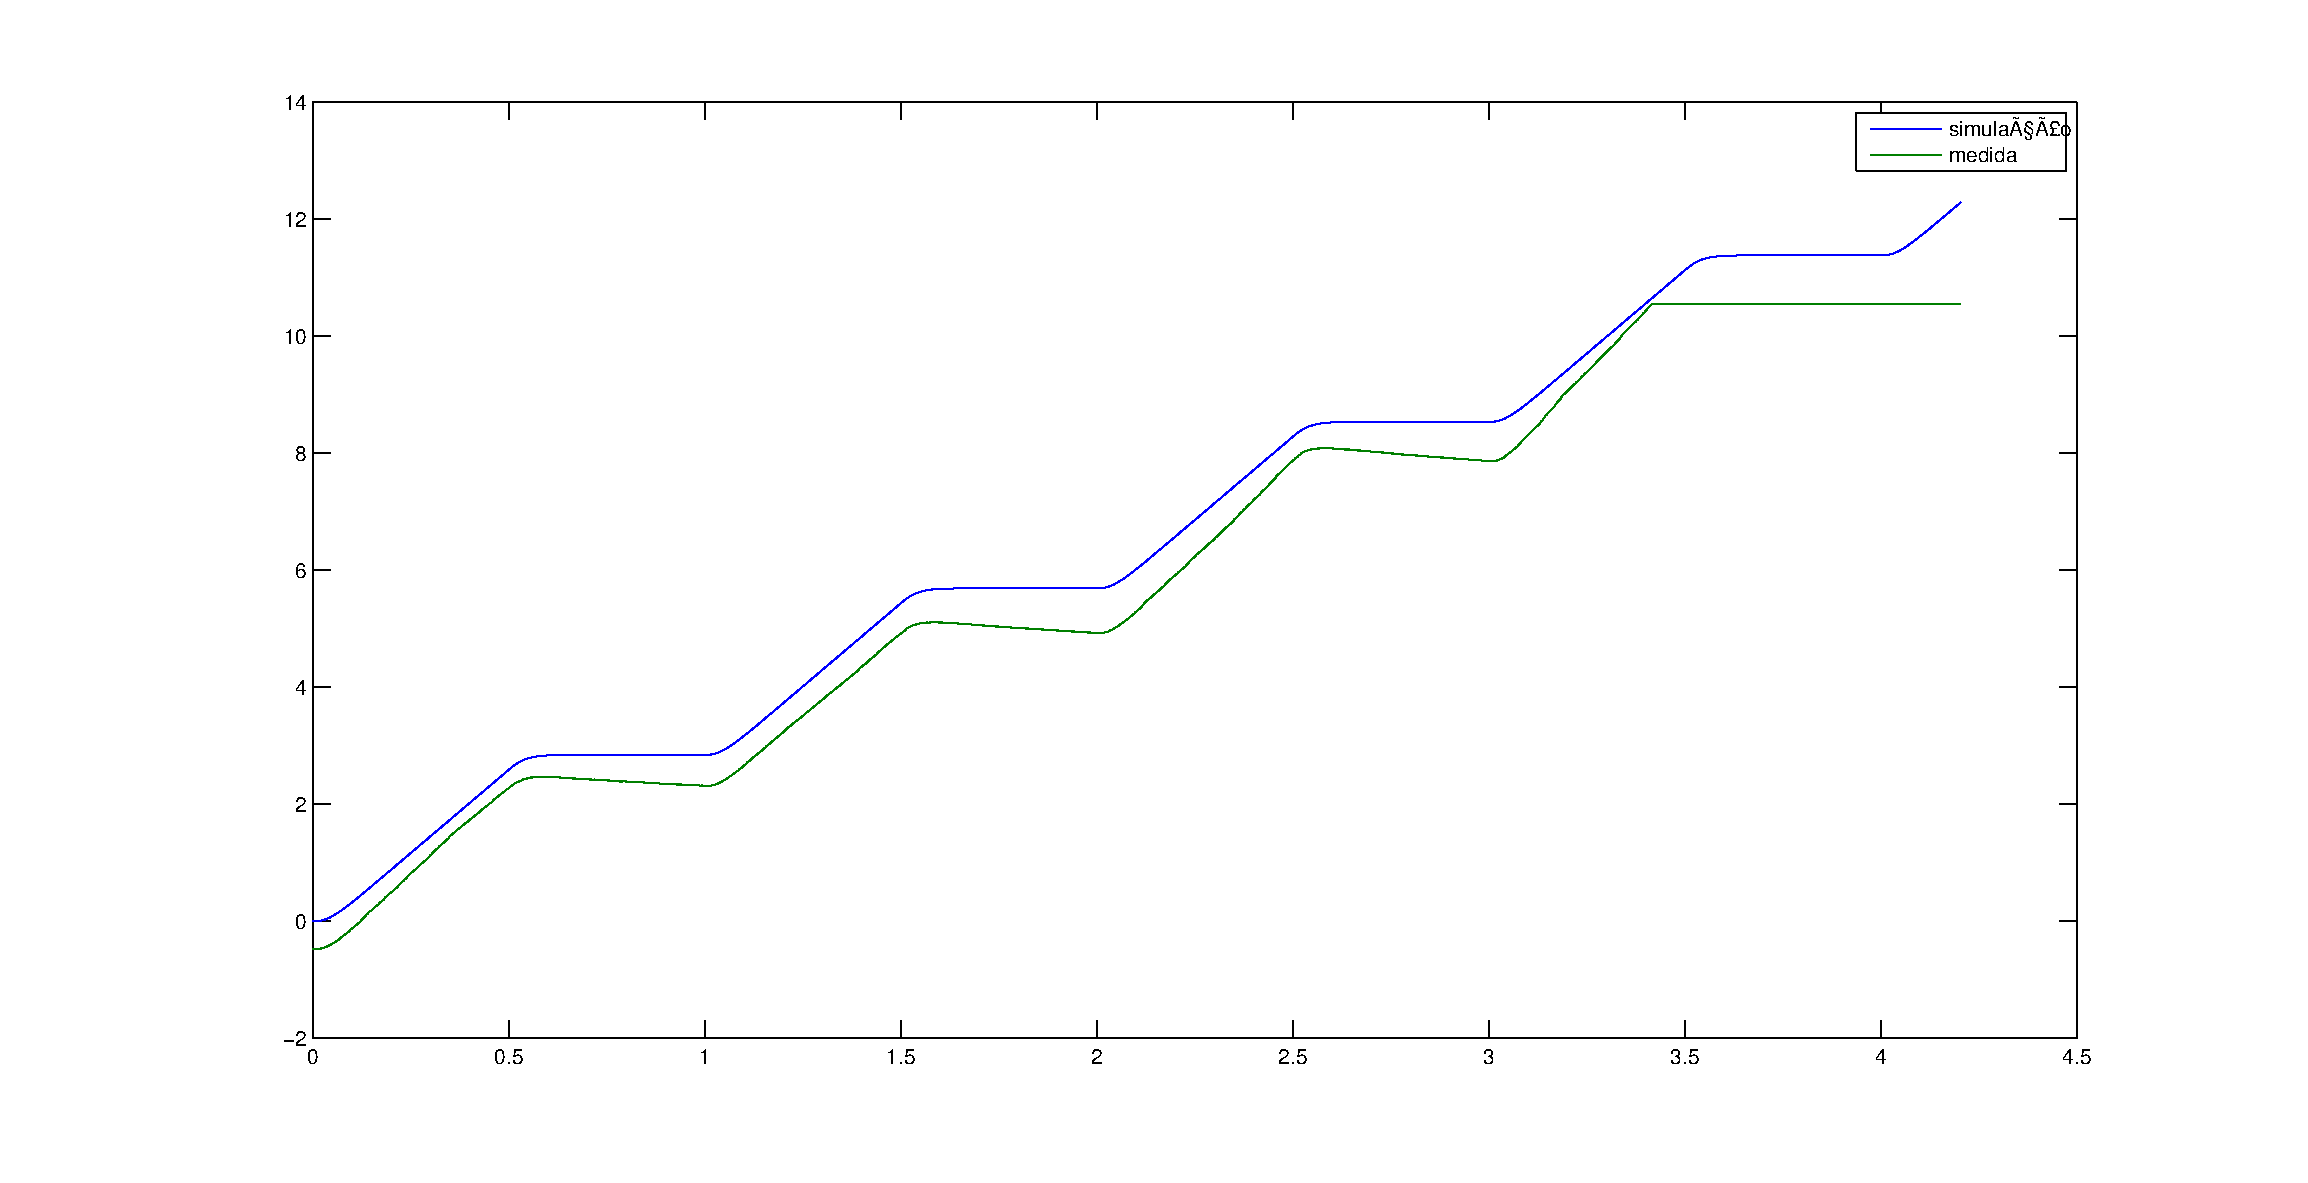
\includegraphics[width=0.8\linewidth]{sim4}
	\caption{Resposta do quarto estágio à uma onda quadrada e simulação da mesma}
	\label{fig:sim4}
\end{figure}

\begin{thebibliography}{widestlabel}
	\bibitem{bb:roteiro}{Roteiro do experimento disponibilizado para os alunos}
\end{thebibliography}
\tiny{Este documento foi formatado utilizando \LaTeX}
\end{document}

